%----------------------------------------------------------------------------------------
%	PACKAGES AND OTHER DOCUMENT CONFIGURATIONS
%----------------------------------------------------------------------------------------

\documentclass[letter,11pt]{scrartcl}

% Fonts, Line-Spacing, and Indentation
\usepackage{fourier}
\usepackage[T1]{fontenc}
\usepackage{microtype}
\usepackage{color}
\setlength\parindent{0pt}
\usepackage{booktabs}
\usepackage{hyperref}
\usepackage{titlesec}
\usepackage[hang,small,labelfont=bf,up,textfont=it,up]{caption}

%------------------------------------------------------

% Symbols
\usepackage{amssymb,amsmath,amsthm}
\usepackage{MnSymbol}
\providecommand{\abs}[1]{\lvert#1\rvert}
\providecommand{\norm}[1]{\lVert#1\rVert}

%------------------------------------------------------

% Sections and Margins
\usepackage{chngcntr}
\usepackage{scrextend}

%------------------------------------------------------

% Venn Diagrams and Images
\usepackage{tikz}
\usetikzlibrary{arrows,backgrounds,petri,shapes,topaths}
\usepackage{float}
\usepackage{wrapfig}

%------------------------------------------------------

% Margins
\usepackage[hmarginratio=1:1,top=10mm,columnsep=20pt]{geometry}

%------------------------------------------------------

% Custom Theorem Setup
\newtheorem{innercustomthm}{Theorem}
\newenvironment{customthm}[1]
  {\renewcommand\theinnercustomthm{#1}\innercustomthm}
  {\endinnercustomthm}


%------------------------------------------------------

% Custom macros
\newcommand{\inlinecode}{\texttt}


%----------------------------------------------------------------------------------------
%	TITLE SECTION
%----------------------------------------------------------------------------------------

\title{
  \normalfont \normalsize
  \textsc{Data Structures - CS 261 (Spring 2015)} \\
  \huge Assignment \#3 -- Part 2
}

\author{Keeley Abbott
\\ Theodore Duchow-Pressley}

\date{\normalsize\today}

%------------------------------------------------------

\begin{document}

\maketitle

%----------------------------------------------------------------------------------------
%	ARTICLE CONTENT
%----------------------------------------------------------------------------------------

\subsection*{1. Which of the implementations uses more memory? Explain why.}

The Linked List implementation uses more memory, because each link contains
space for two addresses (next and previous), as well as the value. Whereas the
Dynamic Array implementation simply contains a contiguous block of memory, full of data.

\begin{figure}[H]
  \centering
  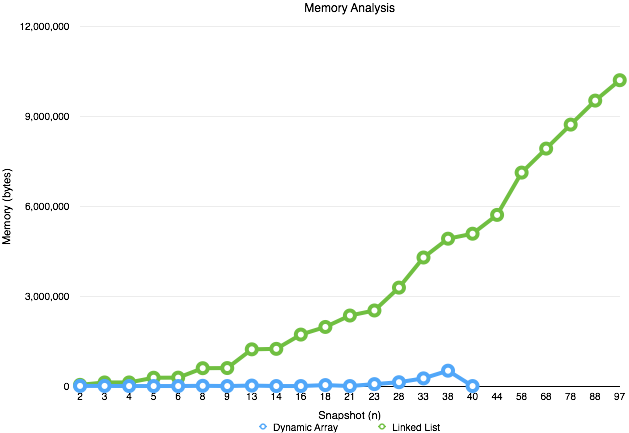
\includegraphics[width=0.5\textwidth]{memory}
  \caption{Memory Allocation Comparison}
\end{figure}

%------------------------------------------------------

\subsection*{2. Which of the implementations is the fastest? Explain why.}

In theory the Linked List implementation should be faster, but in practice the
Dynamic Array implementation is faster. This is because the Dynamic Array
implementation does fewer operations and is able to randomly access items.

\begin{figure}[H]
  \centering
  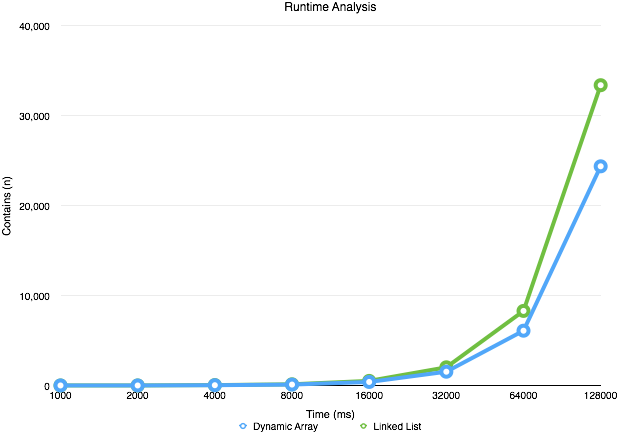
\includegraphics[width=0.5\textwidth]{runtime}
  \caption{Runtime Comparison}
\end{figure}

%------------------------------------------------------

\subsection*{3. Would you expect anything to change if the loop preformed
  \texttt{remove()} instead of \texttt{contains()}? If so, what?}

If we were to change the loop to \texttt{remove()} instead of
\texttt{contains()}, the Linked List would become faster, because removing an
item from a Linked List can be done in O(1) time. Versus removing an item at
any position except the last element of a Dynamic Array taking O(n) time --
because when removing an element in any other position in the Dynamic Array
requires shuffling all other items to fill the gap.

%------------------------------------------------------

\end{document}

%%% Local Variables:
%%% mode: latex
%%% TeX-master: t
%%% End:
